\documentclass[10pt]{article}
\usepackage[utf8]{inputenc}
\usepackage[T1]{fontenc}
\usepackage{fixltx2e}
\usepackage{graphicx}
\usepackage{grffile}
\usepackage{longtable}
\usepackage{wrapfig}
\usepackage{rotating}
\usepackage[normalem]{ulem}
\usepackage{amsmath}
\usepackage{textcomp}
\usepackage{amssymb}
\usepackage{capt-of}
\usepackage{hyperref}
\renewcommand{\baselinestretch}{1.2}
\usepackage[T1]{fontenc}
\usepackage[none]{hyphenat}
\linespread{1.05}
\usepackage[scaled]{helvet}
\usepackage{courier}
\usepackage{titlesec}
\author{John Murray, Michael Mateas, Noah Wardrip-Fruin}
\date{\today}
\title{Toward Analyzing Semantic Structures in Choice-Based Games}
\hypersetup{
 pdfauthor={John Murray, Michael Mateas, Noah Wardrip-Fruin},
 pdftitle={Toward Analyzing Semantic Structures in Choice-Based Games},
 pdfkeywords={},
 pdfsubject={},
 pdfcreator={Emacs 25.0.90.3 (Org mode 8.3.4)}, 
 pdflang={English}}
\begin{document}

\maketitle
\section{Abstract}
\label{sec:orgheadline1}
This paper introduces an approach to modeling interactive choice-based
narratives that extends David Elson's Story Intention Graph to address
choice-based narratives. The goal is to model key content
relationships that may influence important decisions and show the
semantic relationship with past content, even without change in how
the plot progresses or content is selected. It proposes analyzing an
existing non-textual game using tools designed for textual narratives
and situates the approach within the goals of the interactive
storytelling community.
\section{Introduction}
\label{sec:orgheadline2}
The value of a story can be seen as the experience it creates when it
is interpreted by a reader. Interactive storytelling uses the
capabilties of computational media to broaden the number of possible
stories by either branching a story based on player input or
dynamically adjusting the story content based on a simulation (as in
Prom Week \cite{McCoy2013}). These narratives can be in any of a
variety of immersion levels: text-based were popularized as the genre
of interactive fiction, whereas more dramatic interactive stories have
been produced including the interactive drama Facade
\cite{Mateas2005}. 

This paper proposes analyzing commercially available games to better
understand why they present compelling narrative choices. The main
research question is how to model key narrative relationships between
content choices and the experience of a decision.

The paper is organized as follows. We define narrative and
narratology, focusing on the Story Intention Graph. We then define
cinematic choice-based adventure games and describe why it is
suitable. We present a preliminary prototype that allows navigating
content, along with a method of attempting to apply a SIG encoding to
a choice-based game. We conclude with a description of the planned
study and future work.

\section{Modeling Branching Narrative}
\label{sec:orgheadline3}
Narrative can be understood as a phenomena that arises from the
coordination of inherent mental abilities, including the ability to
understand the interaction of agents, their goals, and beliefs and the
sequence of causally related events they are involved in. There is a
long history of its study in the field of narratology. 

Interactive digital narratives represent a possibility space of
potential stories which require non-trivial effort to "experience."
Espen Aarseth calls these works "ergodic literature" in his book,
\emph{Cybertext} \cite{Aarseth1997}, drawing attention to the properties
that differentiates this medium from other types of literature. Nick
Montfort uses the term "traversal" \footnote{One recent Telltale Games work, Minecraft, uses a sandbox-style
creation game based on voxels as its basis, which departs from
previous works that use either comics or television.
;} to describe one possible or
actual story that results from engaging with a work. Hartmut Koenitz
proposed the term "instance" to describe a parameterized traversal,
using the sense prevalent in computer programming \cite{Hartmut2015}.
Koenitz describes the space of instances as a "protostory." 

The Story Intention Graph (SIG) schemata was developed by David Elson
as a set of discourse relations to represent key relationships among
concepts present in textual narratives using concepts from narrative
theory. It does so through three layers: a textual layer, which
contains relevant (but not exhaustive) spans of text from the source
textual story. These are connected to a set of propositions and states
in a layer that captures the described happenings. Finally, there is
an interpretive layer, where propositions are linked to agent goals,
plans and values. Elson collected a set of these SIG encodings of a
set of Aesop’s Fables in order to evaluate the suitability of the
schemata for discovering patterns and similarities among different
stories that went beyond the surface text. He found that the SIG
schemata, even without representing individual propositions, was more
successful than alternative methods at identifying similarities in the
stories.

We focus our attention on a subgenre of cinematic choice-based
adventure games. These games are relatively hand-authored and rely on
a series of choices dramatically presented to players. They represent
is an opportunity to understand story and interactivity in a genre
that can be made constrained so as to be tractable for computational
narratology approaches.

This subgenre is an example of a branching narrative, the most common
way of reading and executing non-linear stories. There are a number of
tools now available to create narratives based on a model of lexia and
links, including Ink, Twine, Ren'Py and ChoiceScript. These tools
enable authors to create textual or visual narratives with various
mechanisms to direct the player along particular paths, or traversals.

\section{Methodology and Problem Analysis}
\label{sec:orgheadline4}
There are two distinct challenges to developing and testing a model
for the subgenre of Cinematic choice-based adventure games. First, the
media is fundamentally visual and dramatic, whereas the tools designed
for both authorship (in the case with Twine and Ink) are textual as
well as modeling (Elson's authoring tool, \emph{Scheharazade}
\cite{Elson2012}). Second, the chosen model was designed for a linear
narrative. The non-textual nature of the media presents a number of
obstacles to analysis, including the difficulty in quickly navigate
across choice paths while viewing content either within the game
engine or on complete recordings. 

The first content exploration issue was addressed by creating a
web-based content browser that enables a user to change the choice at
each points and see the resulting changes in the content.

\begin{figure}[htb]
\centering
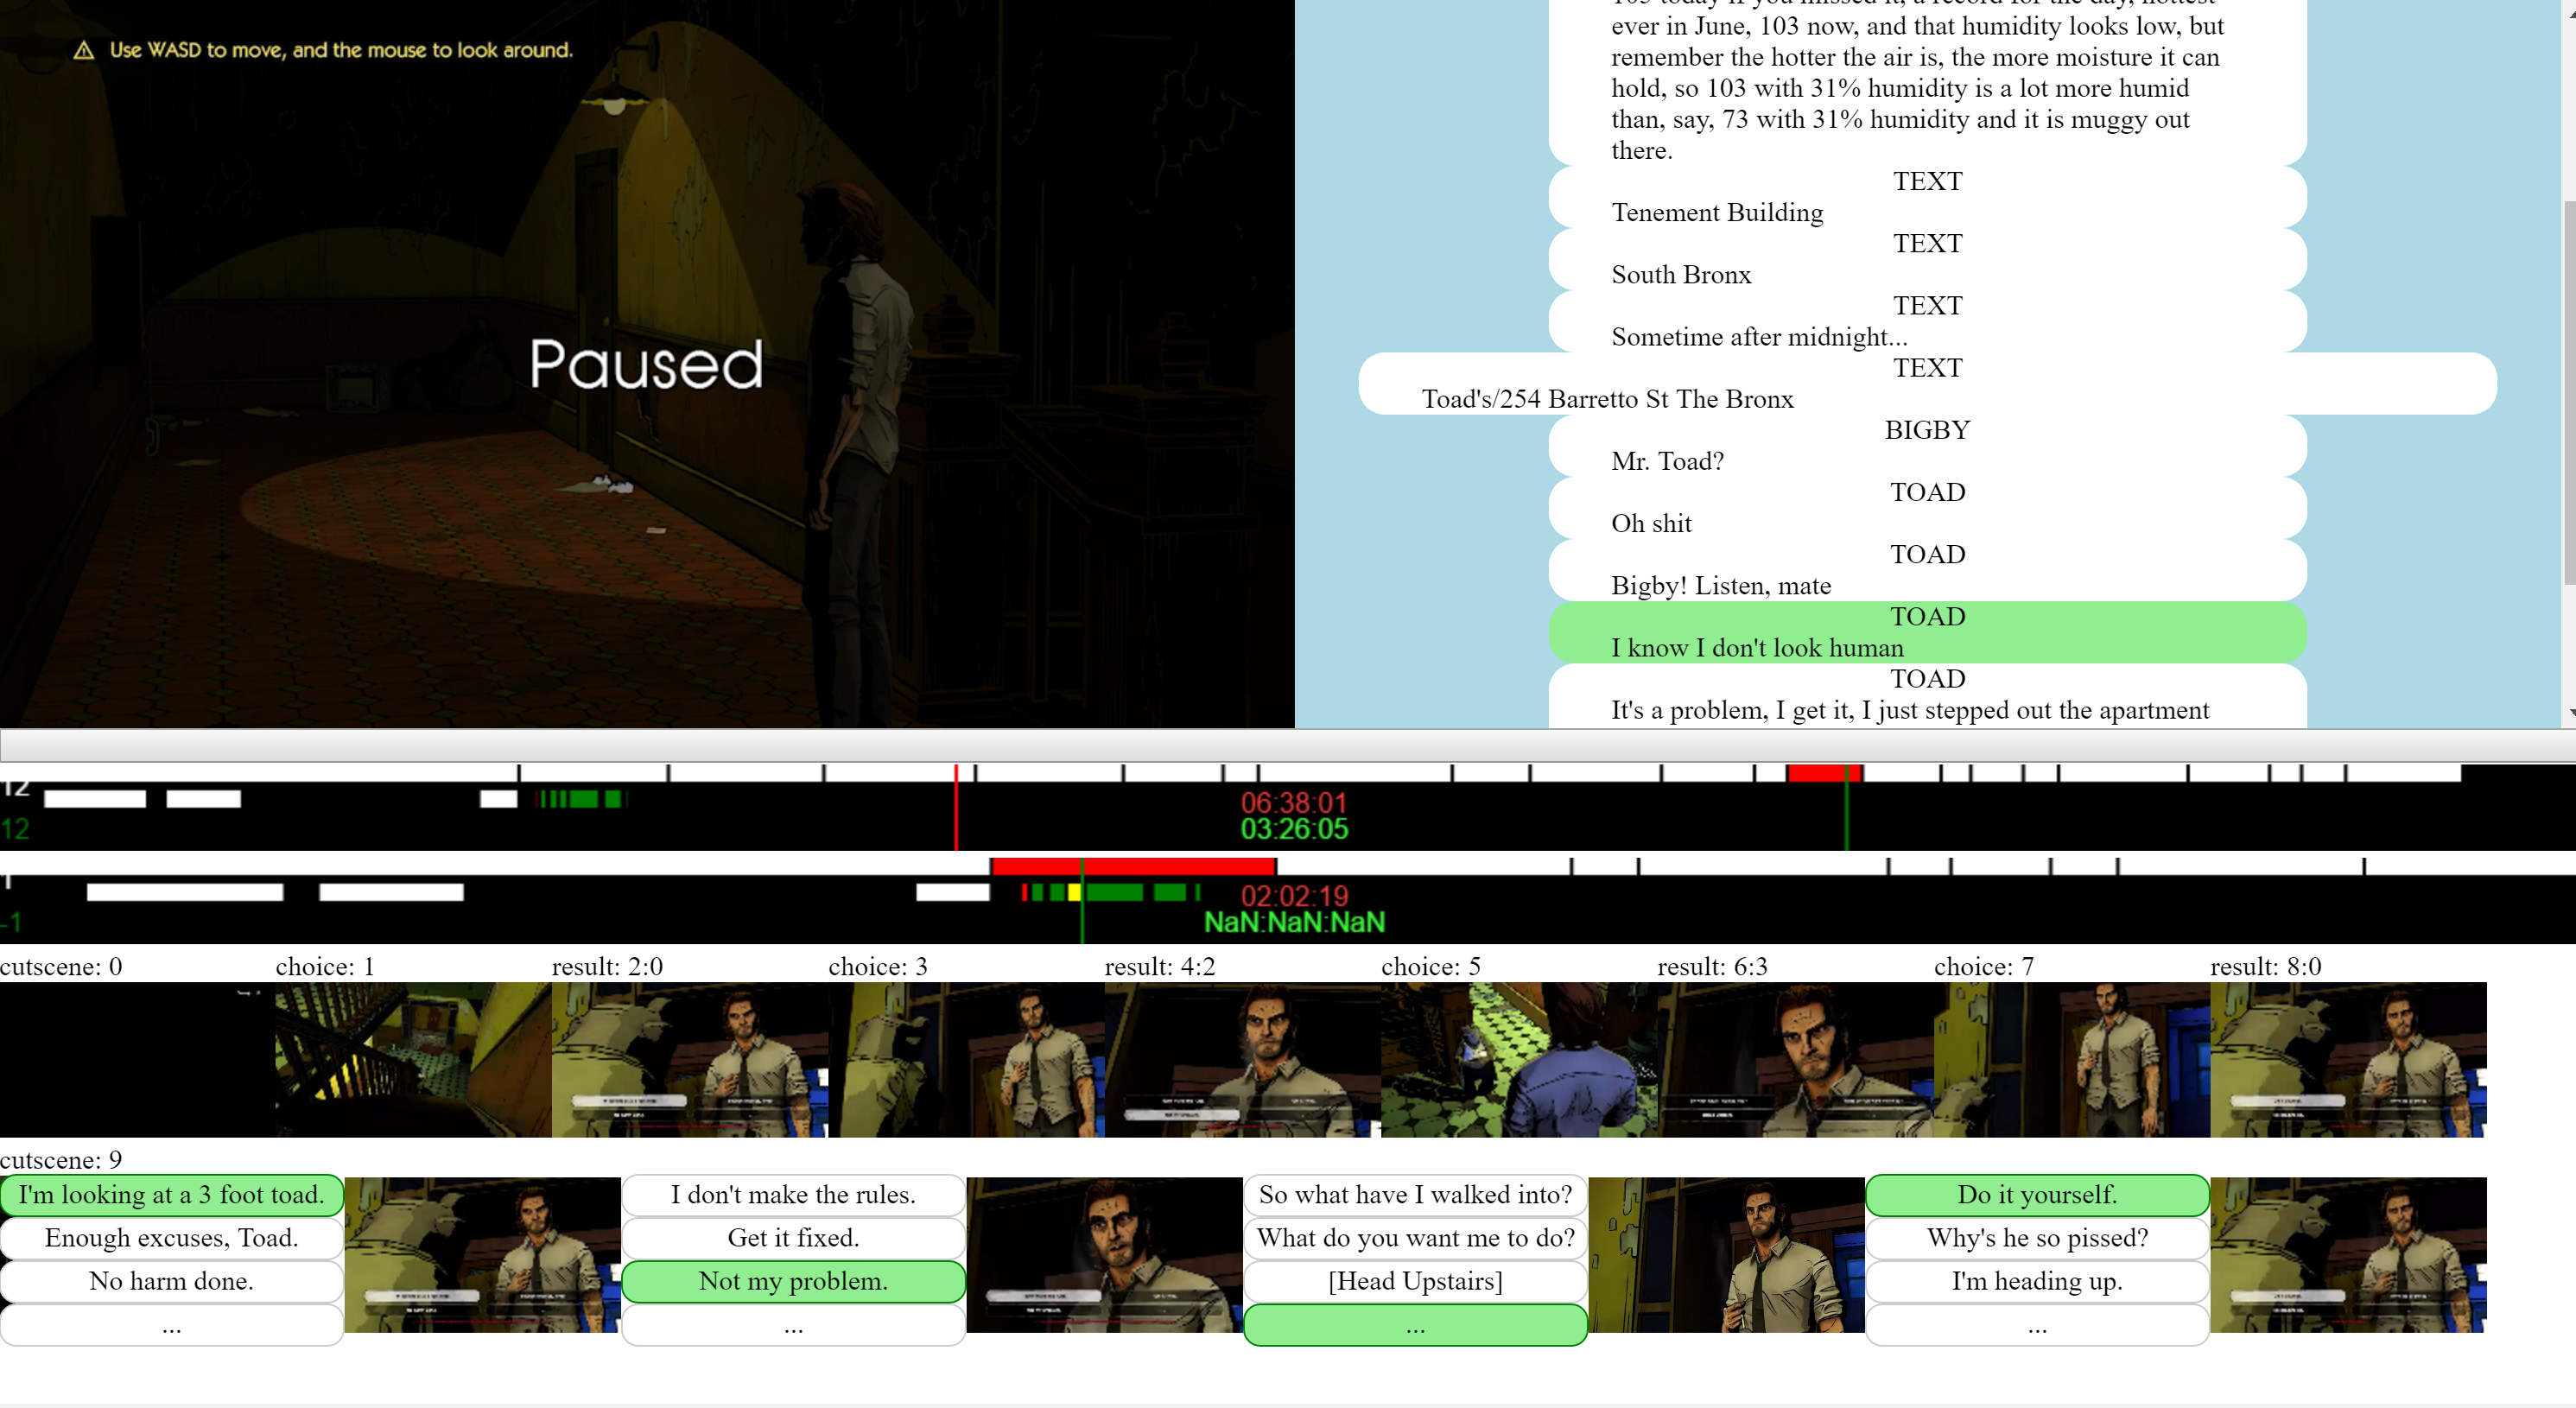
\includegraphics[width=.9\linewidth]{story_browser.png}
\caption{Story Browser Prototype Interface}
\end{figure}

The Story Browser Interface shows off two main features: 

\begin{enumerate}
\item A navigation timeline that shows the location of segments of
content, both raw and traversal-specific.
\item A choice selection interface to specify choices "selected."
Selections change the sequence to play content including that
result.
\end{enumerate}

The second challenge is by far more important and central to the
proposed work. A diagram of the various content segments and their
branches is insufficient to understanding how seemingly "unimportant"
choices can influence the perception of a character during key
decisions. An example: Bigsby can treat Toad two different ways in the
opening scene. This causes two distinct content options in a later
conversation as a result from this initial choice, but the perception
of the relationship is defined by the reactions.

These value-specific changes that converge quickly are exactly the
sort of variations that games in the genre are known for, and are
poorly modeled by a pure structural approach.

In order to decide on which extensions are necessary to the SIG, we
first attempted to reduce the game's media presentation into a textual
script with key emotes and descriptions included. We knew that a
choice-based authoring tool could capture the variations present in
the game, including tracking of certain key choices and the display of
optional content in free-roam modes. Ink by InklStudios
(\url{https://github.com/inkle/ink}) was selected. It was open source,
produced a json data file and its source file was human readable and
could be annotated within the existing SIG annotation tool,
Scheharazade.

\section{Future Work}
\label{sec:orgheadline5}
The proposed work will compile a corpus of encodings and evaluate
whether the graphs are predictive of which content corresponds to
which decision. By better understanding what works using existing
tools, we can better understand both how to develop better content,
how to understand how existing artifacts create the effects that they
do and further anticipate how to create more efficient and powerful
authoring tools and systems.

\section{References}
\label{sec:orgheadline6}
\bibliographystyle{plain}
\bibliography{../../../library}
\end{document}
